\section{Conception}

\todoGeneric{10 à 15 pages de conception}

\todoGeneric[inline]{Intro de la section conception}

\subsection{Robot}

\subsubsection{Électronique}
\todoWho{Jordan}

\todoPoints{Vous y joindrez tous les documents nécessaires (croquis, schémas électriques, ordinogrammes, calculs, etc.) pour expliquer vos choix.}
\todoPoints{Justifier vos choix.}
\todoPoints{Mentionner les performances et les limitations du prototype.}
\todo{Bluetooth}

\subsubsection{Logiciel}
\todoWho{Thierry}

\todoPoints{Vous y joindrez tous les documents nécessaires (croquis, schémas électriques, ordinogrammes, calculs, etc.) pour expliquer vos choix.}
\todoPoints{Justifier vos choix.}
\todoPoints{Mentionner les performances et les limitations du prototype.}

\subsubsection{Mécanique}
\todoWho{Will}

Le lanceur de balles est une partie très importante du projet,
car il doit être capable de faire ce qu’il est conçu de façon consistante pour faciliter son utilisation.
Il se sépare en 3 parties principales:
la partie propulsion,
la partie recharge ainsi que
la partie visé.

\subsubsection{Mode de propulsion}
Pour la propulsion de la balle, trois systèmes ont été étudiés pour assurer une certaine précision tout en gardant le système simple.

\paragraph{Option 1: par contact}
Nous avons pensé à un système comprimant un ressort à l’aide d’un boîte de vitesse et d’une crémaillères.
Ce système à vite été écarté puisque nous ne savions pas si les pièces, principalement imprimées en PLA, allaient être capable de supporter l'énergie emmagasinée dans le ressort.
De plus, il aurait fallu avoir une façon de placer les balles à la bonne distance du ressort et les faire tenir en place avant le contact, ce qui aurait compliqué les choses rapidement.
Un solénoïde à aussi été envisagé pour frapper la balle, mais nos connaissance en magnétisme n’étaient pas adéquates pour considérer cette option plus sérieusement.

\todo{(Placer photo croquis)}

\paragraph{Option 2.1: par piston}
Un système comparable à ce que l’on retrouve dans les jouets de type “Airsoft” à aussi été étudié.
Ce système consiste encore une fois à comprimer un ressort attaché à un piston pour créer une différence de pression entre le devant et le derrière de la balle, la propulsant vers l’avant.
Ce système comporte les mêmes désavantages que la première option, en plus des problèmes d’étanchéité que peuvent apporter les pièces imprimées.
Il a donc été écarté.

\paragraph{Option 2.2: par air comprimée.}
Nous avons pensé à remplacer le piston par une pompe à air et un réservoir pressurisé.
Sachant que l’air comprimé peut être très dangereux si le système échoue, et que nous allions être en présence de famille lors des démonstrations, cette option était donc une mauvaise idée.
De plus, un système comme celui-ci aurait été beaucoup plus compliqué que le système final choisi.
\todo{(Placer photo croquis)}

\paragraph{Choix final: Roue d’inertie.}
Nous avons donc opté pour une roue d’inertie pour propulser nos balle.
L’idée est venue des jouets de la marque NERF, qui utilisent 2 roues tournant en sens inverse pour propulser des fléchettes de mousse sur une distance acceptable.
Ce système est aussi assez simple, puisqu’il requiert seulement un moteur pouvant tourner à une vitesse contrôlable et d’une roue d’inertie.
Dans les lanceurs NERF, les roues étaient en plastique dur, puisque que les projectiles étaient en mousse molle et très malléable.
Dans notre cas, nous ne voulions pas briser la balle, il a donc fallu rajouter une extérieure de mousse servant à isoler les cadres de portes.

\todo{(Placer photo de la roue)}

\subsubsection{Méthode de chargement de la balle}
Quelques méthode pour pousser les balles vers la roue d’inertie ont étés envisagées.
Voici les trois options principales.

\paragraph{Option 1: Par gravité}
Nous avons pensé à utiliser la gravité pour pousser les balles sous la roue d’inertie pour simplifier le système.
ce système aurait seulement eu besoin d’un servo pour assurer qu’une seule balle tombe à la fois dans le lanceur.
Cependant, le système de roue d’inertie fait que la distance entre la roue et la base du lanceur est plus petit qu’une balle (pour que la balle soit pressée dans la mousse, assurant un transfert d’énergie suffisant pour la propulser.
La gravité n’avait donc pas la force nécessaire pour enfoncer la balle sous la roue.

\paragraph{Option 2: came et tige-poussoir.}
Nous voulions nous servir d’un servo pour gérer le chargement, car ils sont simple à utiliser et assez précis pour nos besoins.
Le débattement nécessaire pour amener les balles de la position ou les balles sont placées jusqu’en dessous de la roue est d’environ 75 mm (les balles faisant 40mm de diamètre et en ajoutant quelques millimètres pour assurer la solidité du lanceur).
Les servos allant seulement de 0 à 180 degrés, il aurait fallu une camme d’au moins 75 mm de diamètre pour accommoder ce débattement, ce qui aurait été beaucoup trop gros en comparaison au lanceur.

\paragraph{Option 3: pignon et crémaillère}
Cet option est parfaite, puisqu’elle règle le seul problème que la came avait: la dimension des roues.
En se servant des CADs fournies par McMaster.com, il a été facile de trouver des pièces de dimensions adéquates pour notre système.
Un pignon ayant un diamètre primitif de 1 pouce ayant 20 dents et sa crémaillère répondaient parfaitement à nos critères de dimensions.
Il nous faudrait donc faire tourner le pignon une fois(2*pi*0,5 po) pour atteindre le débattement voulu (3po).
Il fallait donc changer 180 degrés du servo en 360 degré.
Nous avons donc utilisé deux roues ayant le même diamètre primitif que la première, dont une avait 2 fois plus de dents pour assurer un tour complet.
Les roues de 12 et 24 dents ont donc étés choisies car elles etait de bonne dimensions.

\begin{figure}[h!]
    \centering
    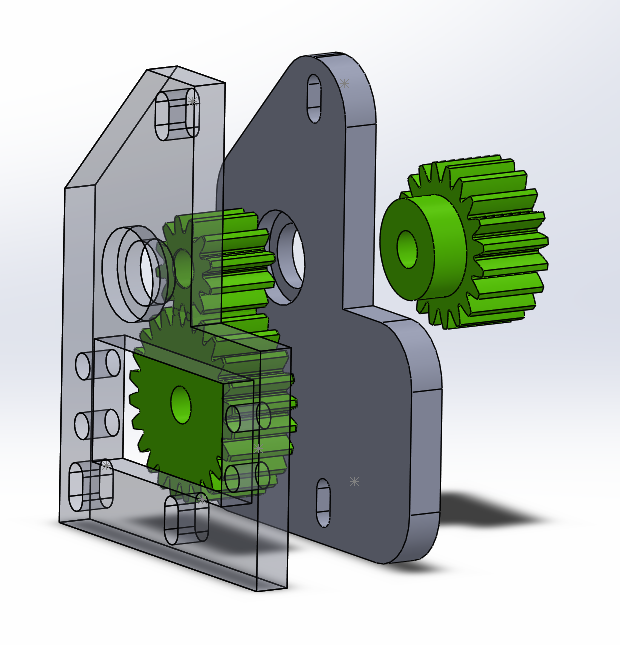
\includegraphics[width=0.5\linewidth]{img/s2/cad/gearbox1.PNG}
    \caption{Description de l'image.}
    \label{fig:s2-cad-gearbox1}
\end{figure}
\todo{add a description to the figure}

\subsubsection{Mode de visé}
Plusieurs options s’offraient à nous pour visé avec le lanceur.
La première étant de jouer avec l’angle du lanceur pour aller chercher différentes distance (pour atteindre tous les verres de beer pong).
Cette option a été écartée puisque nous ne savions pas le poids finale du lanceur et si un servo allait être capable de le maintenir en place de façon constante.
Nous avons donc conçue un un support ayant un arc de cercle ce qui nous a permit de choisir une angle et de sécuriser le lanceur à cet angle.

\missingfigure{support de visé}
La distance des lancers allait donc être déterminée par la vitesse à laquelle la roue d’inertie tourne, ainsi que la pression qu’elle applique sur les balles.

\subsubsection{Version finale}
La version finale allait donc être un lanceur fixe rechargé par une crémaillère, qui propulse les balles à l’aide d’une roue d’inertie.
Notre Première itération comportait une grande rampe pour assurer que les balles aient un maximum de temps en contact avec le lanceur pour augmenter la précision.
Cette idée de rampe a été abandonnée lorsque nous avons réalisé de qu’elle ampleur elle devait être pour répondre à nos besoins (un arc de cercle d’environ 150 mm de rayon, pour assurer un arc de cercle assez graduel.
Nous avons donc optés pour un lancer direct avec un petit canon pour réduire les imprécisions de la roue.

\missingfigure{Rampe de lancement}
fig:Rampe de lancement
\begin{figure}[h!]
    \centering
    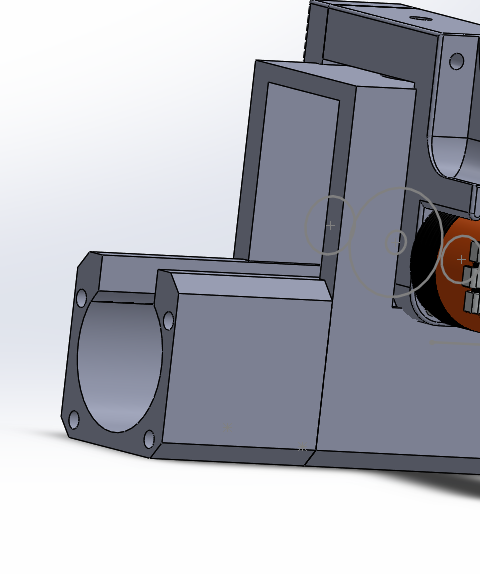
\includegraphics[width=0.5\linewidth]{img/s2/cad/cannon.PNG}
    \caption{Description de l'image.}
    \label{fig:s2-cad-cannon}
\end{figure}
\todo{add a description to the figure}


Une autre amélioration de la version finale à été de fixer l’axe de la roue d’inertie des deux côtés et d’ajouter un roulement à bille.
Les pièces imprimées en 3D sont rarement balancées et la roue ajoutait beaucoup de vibration au système.
Le roulement à bille réduisait aussi la friction entre l’arbre de la roue et le support en plastique, qui avait tendance à fondre durant l’utilisation.
De plus, ce support facilitait aussi l’ajustement de la position de la roue d’inertie.
Un écrou sous le support était facilement accessible et nous n’avions plus besoins de défaire le montage au complet pour dévisser le moteur et changer sa hauteur.
Ce support était aussi imprimé en 2 pièces pour faciliter son implémentation au système.

\begin{figure}[h!]
    \centering
    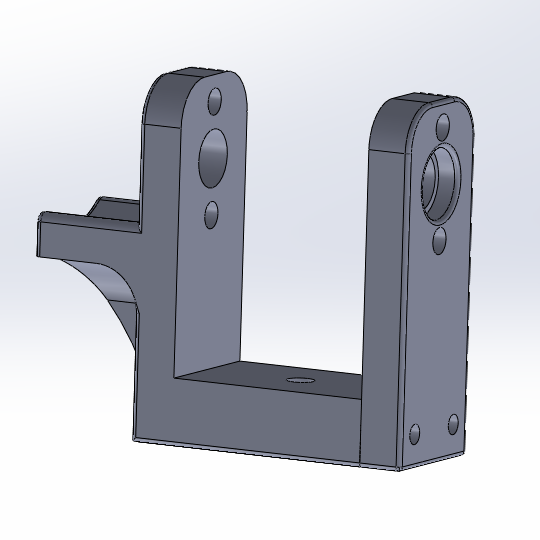
\includegraphics[width=0.5\linewidth]{img/s2/cad/motorholer.PNG}
    \caption{Description de l'image.}
    \label{fig:s2-cad-motorholer}
\end{figure}
\todo{add a description to the figure}

\todo{ajouter photo}

Pour assurer un maillage adéquat entre les roues de la boîte de transmission et la crémaillère, des trous oblongs avaient étés utilisés.
Cependant, Nous nous sommes rendu compte que ces trous ne servaient pas à grand chose et que les engrenages devaient être plus contraintes.
La position du servo a aussi été modifiée puisqu’il interférait avec les tiges filetées servant à fixer le système.
Nous avons donc conçue une boîte de transmission complètement indépendante du lanceur et qui gardait toujours la bonne distance entre les engrenages.
Cette boite était par la suite fixée au lanceur à l’aide des trous prévus à cette effet.

\begin{figure}[h!]
    \centering
    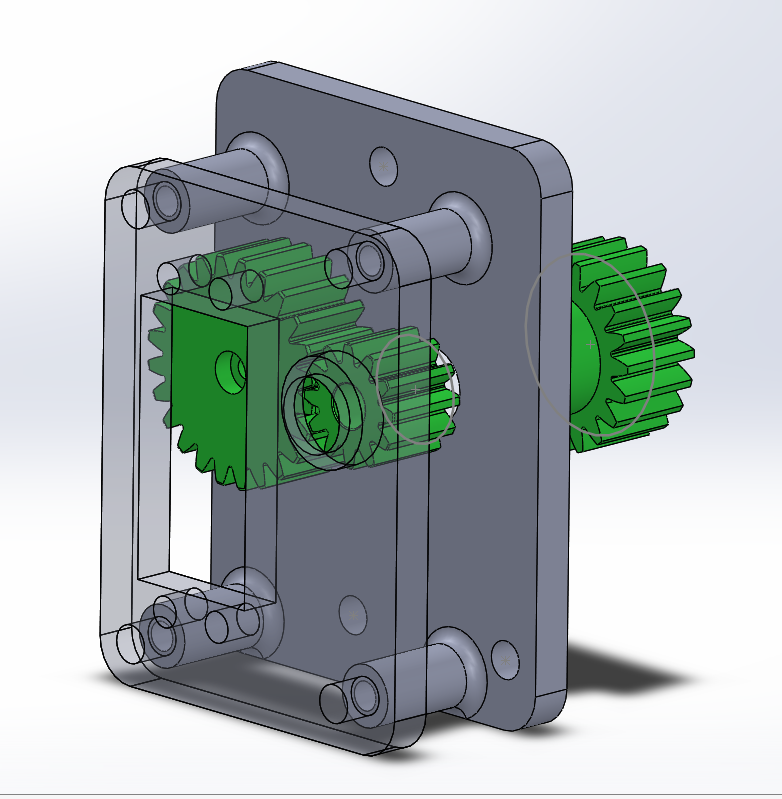
\includegraphics[width=0.5\linewidth]{img/s2/cad/gearbox2.PNG}
    \caption{Description de l'image.}
    \label{fig:s2-cad-gearbox2}
\end{figure}
\todo{add a description to the figure}

\todo{ajouter photo}
Le PLA est un plastique malléable et facile à percer.
Nous nous sommes servis de ces caractéristique pour décortiquer notre lanceur en pièces faciles à imprimer et nous avons utilisés des tiges filetées de dimensions 10-32 pour tenir le tout ensemble.

\begin{figure}[h!]
    \centering

    \begin{subfigure}{0.4\linewidth}
        \centering
        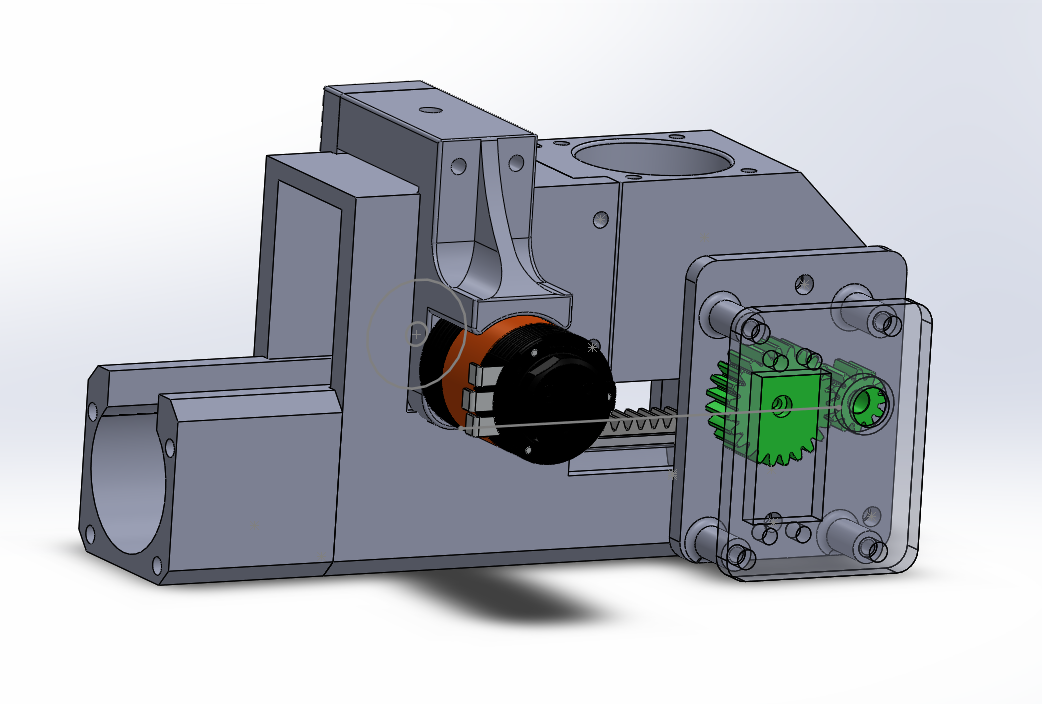
\includegraphics[width=\linewidth]{img/s2/cad/lanceur1.PNG}
        \caption{Description de l'image.}
        \label{fig:a1-s2-cad-lanceur1}
    \end{subfigure}
    \begin{subfigure}{0.4\linewidth}
        \centering
        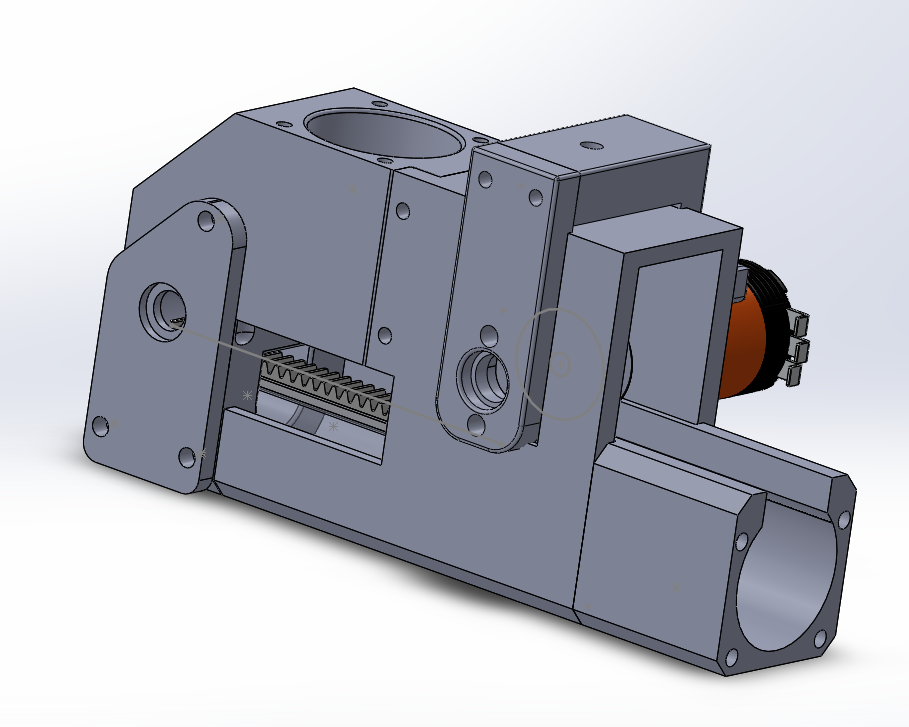
\includegraphics[width=\linewidth]{img/s2/cad/lanceur2.PNG}
        \caption{Description de l'image.}
        \label{fig:a1-s2-cad-lanceur2}
    \end{subfigure}

    \caption{Description de l'image.}
    \label{fig:template-example-flottante}
\end{figure}
\todo{add a description to the figure}

\todo{ajouter photo monté}

\subsection{Verre}

\subsubsection{Électronique}
\todoWho{Vincent}

\todoPoints{Vous y joindrez tous les documents nécessaires (croquis, schémas électriques, ordinogrammes, calculs, etc.) pour expliquer vos choix.}
\todoPoints{Justifier vos choix.}
\todoPoints{Mentionner les performances et les limitations du prototype.}

\subsubsection{Logiciel}
\todoWho{Thierry}

\todoPoints{Vous y joindrez tous les documents nécessaires (croquis, schémas électriques, ordinogrammes, calculs, etc.) pour expliquer vos choix.}
\todoPoints{Justifier vos choix.}
\todoPoints{Mentionner les performances et les limitations du prototype.}


\subsubsection{Mécanique}
\todoWho{Vincent}

\todoPoints{Vous y joindrez tous les documents nécessaires (croquis, schémas électriques, ordinogrammes, calculs, etc.) pour expliquer vos choix.}
\todoPoints{Justifier vos choix.}
\todoPoints{Mentionner les performances et les limitations du prototype.}

\subsection{Application}

\subsubsection{Logiciel}
\todoWho{Thierry}

\todoPoints{Vous y joindrez tous les documents nécessaires (croquis, schémas électriques, ordinogrammes, calculs, etc.) pour expliquer vos choix.}
\todoPoints{Justifier vos choix.}
\todoPoints{Mentionner les performances et les limitations du prototype.}
